\documentclass{article}

\usepackage[margin=1in]{geometry}
\usepackage{amsmath,amsthm,amssymb}
\usepackage{bbm, enumerate, tikz}
\usepackage{multicol}

\newenvironment{problem}[2][Problem]{\begin{trivlist}
\item[\hskip \labelsep {\bfseries #1}\hskip \labelsep {\bfseries #2.}]}{\end{trivlist}}
\newenvironment{note}[1][Note.]{\begin{trivlist}
\item[\hskip \labelsep {\bfseries #1}]}{\end{trivlist}}

\begin{document}

\title{Complex Analysis: Homework 13}
\author{Peter Kagey}

\maketitle

% -----------------------------------------------------
% Problem
% -----------------------------------------------------
\begin{problem}{3} (page 206) \\
  The formula (42) permits us to evaluate the \textit{probability integral} \begin{align}
    \int_0^\infty e^{-t^2} dt
      = \frac{1}{2} \int_0^\infty e^{-x}x^{-1/2} dx
      = \frac{1}{2} \Gamma(1/2)
      = \frac{1}{2} \sqrt{\pi}
  \end{align}
  Use this result together with Cauchy's theorem to compute the
  \textit{Fresnel integrals} \begin{align}
    \int_0^\infty \sin(x^2) dx
    = \int_0^\infty \cos(x^2) dx
    = \frac{1}{2}\sqrt{\pi/2}
  \end{align}
\end{problem}
\begin{proof} \text{} \\
  The plan is to use the construction from Wikipedia and integrate
  $f(z) = e^{-z^2}$ along the contour given by \begin{multicols}{2}
  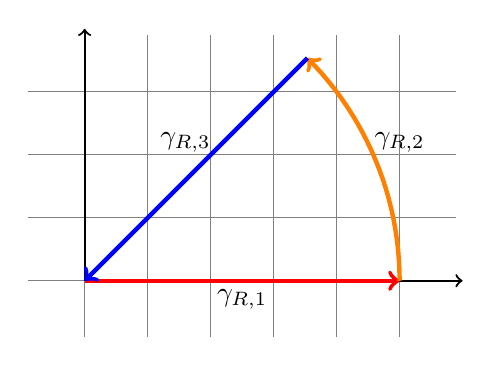
\begin{tikzpicture}[scale=0.8]
    \draw[very thin,color=gray] (-0.9,-0.9) grid (5.9,3.9);
    \draw[thick, ->] (0,0)--(6,0);
    \draw[thick, ->] (0,0)--(0,4);
    \draw[ultra thick, ->, draw=red, domain=0:5] plot ({\x}, {0});
    \draw node at (2.5, -0.3) {$\gamma_{R,1}$};
    \draw[ultra thick, ->, draw=orange, domain=0:45] plot ({5*cos(\x)}, {5*sin(\x)});
    \draw node at (5, 2.2) {$\gamma_{R,2}$};
    \draw[ultra thick, <-, draw=blue, domain=0:5] plot ({\x*cos(45)}, {\x*sin(45)});
    \draw node at (1.6, 2.2) {$\gamma_{R,3}$};
  \end{tikzpicture}\\
  \begin{align}
    \gamma_{R,1} &= \{t + 0i\ |\ x \in [0, R] \} \\
    \gamma_{R,2} &= \{R e^{it}\ |\ t \in [0,\pi/4] \} \\
    \gamma_{R,3} &= \{te^{i\pi/4}\ |\ t \in [0, R]\}.
  \end{align}
  \end{multicols}
  The first integral is known: \begin{align}
    \lim_{R\rightarrow \infty}\int_{\gamma_{R,1}} f(z)\,dz
      = \int_0^\infty e^{-t^2} dt
      = \frac{1}{2}\sqrt{\pi}.
  \end{align}
  The second integral vanishes in the limit, \begin{align}
    \int_{\gamma_{R,2}} f(z)\,dz
      &= iR\int_0^{\pi/4}\exp(-(Re^{it})^2)\cdot e^{it}\,dt.
  \end{align}
  So by looking at the modulus, we get \begin{align}
    \left|\int_{\gamma_{R,2}} f(z)\,dz\right|
    &\leq R\int_0^{\pi/4}|\exp(-R^2e^{2it})| \cdot |e^{it}|\,dt \\
    &= R\int_0^{\pi/4}|e^{-R^2\cos(2t)}|\cdot\underbrace{|e^{-iR^2\sin(2t))}|}_{=1}\,dt.
  \end{align}
  Continuing now with the inequality $\cos(2t) \geq \pi/4 - t$ for $t \in [0, \pi/4]$,
  \begin{align}
    \left|\int_{\gamma_{R,2}} f(z)\,dz\right|
    &\leq R\int_0^{\pi/4}|e^{-R^2(\pi/4 - t)}|\,dt \\
    &= \frac{R}{e^{R^2\pi/4}}\int_0^{\pi/4}|e^{R^2t}|\,dt \\
    &= \frac{R}{e^{R^2\pi/4}}\left[\frac{e^{R^2t}}{R^2}\right]_0^{\pi/4} \\
    &= \frac{R}{e^{R^2\pi/4}}\left[\frac{e^{R^2\pi/4}}{R^2} - \frac{1}{R^2}\right] \\
    &= \frac{1}{R} - \frac{1}{Re^{R^2\pi/4}} \\
    &\leq \frac{1}{R}.
  \end{align}
  Thus \begin{align}
    \lim_{R \rightarrow \infty}\int_{\gamma_{R,2}} f(z)\,dz = 0.
  \end{align}
  Next, the third integral: \begin{align}
    \int_{\gamma_{R,3}} f(z)\,dz
      &= \int_R^0 e^{i\pi/4}\exp(-t^2\underbrace{e^{i\pi/2}}_{=i})\,dt \\
      &= e^{i\pi/4}\int_R^0 e^{-it^2}\,dt \\
      &= e^{i\pi/4}\int_R^0 \cos(-t^2) + i \sin(-t^2)\,dt \\
  \end{align}
  Because $f$ is entire, it follows from Cauchy's theorem that \begin{align}
    \int_{\gamma_{R,1}} f(z)\,dz + \int_{\gamma_{R,2}} f(z)\,dz + \int_{\gamma_{R,3}} f(z)\,dz = 0,
  \end{align} including in the limit, therefore \begin{align}
    \lim_{R\rightarrow \infty}\left(-\int_{\gamma_{R,3}} f(z)\,dz\right)
      &= e^{i\pi/4}\int_0^\infty \cos(-t^2) + i \sin(-t^2)\,dt \\
      &= \frac{1}{2}\sqrt{\pi}.
  \end{align} This means that \begin{align}
    \int_0^\infty \cos(-t^2) + i \sin(-t^2)\,dt
    &= \int_0^\infty \cos(t^2) - i \sin(t^2)\,dt \\
    &= \frac{\sqrt{\pi}}{2e^{i\pi/4}} \\
    &= \left(\frac{1}{2} - \frac{i}{2}\right)\sqrt{\frac{\pi}{2}}
  \end{align}
    so by looking at the real and purely imaginary parts it follows that
    \begin{align}
    \int_0^\infty \cos(t^2)\,dt
      = \frac{1}{2}\sqrt{\frac{\pi}{2}}
      = \int_0^\infty \sin(t^2)\,dt.
  \end{align}
\end{proof}
\pagebreak

% -----------------------------------------------------
% Problem
% -----------------------------------------------------
\begin{problem}{2} (page 212) \\
  Assume that $f(z)$ has genus zero so that \begin{align}
    f(z) = z^m \prod_n \left(1-\frac{z}{a_n}\right).
  \end{align} Compare $f(z)$ with \begin{align}
    g(z) = z^m \prod_n \left(1 - \frac{z}{|a_n|}\right)
  \end{align} and show that \begin{align*}
    \max_{|z|=r} |f(z)| &\leq \max_{|z|=r} |g(z)|, \text{ and} \\
    \min_{|z|=r} |f(z)| &\geq \min_{|z|=r} |g(z)|.
  \end{align*}
\end{problem}
\begin{proof} \text{} \\
  The heuristic for why $g$ is more ``extreme'' is because all of the zeros lie
  on the same ray, the positive part of the real axis. In particular, by
  considering the ratio \[
    \left|\frac{f(z_0)}{g(z_1)}\right|
    = \left|
      \frac{\displaystyle z_0^m \prod_n \left(1-\frac{z_0}{a_n}\right)}
      {\displaystyle z_1^m \prod_n \left(1 - \frac{z_1}{|a_n|}\right)}
    \right|
    = \left|
      \frac{\displaystyle \prod_n \left(a_n - z_0\right)}
      {\displaystyle \prod_n \left(|a_n| - z_1\right)}
    \right|
    =
      \frac{\displaystyle \prod_n \left|a_n - z_0\right|}
      {\displaystyle \prod_n \left||a_n| - z_1\right|}.
  \] where $|z_0| = |z_1| = r$, it can be seen that it is enough to consider
  $\prod_n \left|a_n - z\right|$ and $\prod_n \left||a_n| - z\right|$.
  \\~\\
  By the triangle inequality,
  \begin{align*}
    |a_n - z| &\leq |a_n| + |z| = |a_n| + r \text{ and}\\
    |a_n - z| &\geq |a_n| - |z| = |a_n| - r,
  \end{align*} so in particular, a given linear factor $a_n - z$ is minimized at
  $\displaystyle z = r\frac{a_n}{|a_n|}$ and maximized at
  $\displaystyle z = -r\frac{a_n}{|a_n|}$: \begin{align}
    \left|a_n - r\frac{a_n}{|a_n|}\right|
      = |a_n|\cdot\underbrace{\left|1 - \frac{r}{|a_n|}\right|}_\text{real}
      = |a_n|\left(1 - \frac{r}{|a_n|}\right)
      = |a_n| - r
      \leq |a_n - z|\\
    \left|a_n + r\frac{a_n}{|a_n|}\right|
      = |a_n|\cdot\underbrace{\left|1 + \frac{r}{|a_n|}\right|}_\text{real}
      = |a_n|\left(1 + \frac{r}{|a_n|}\right)
      = |a_n| + r
      \geq |a_n - z|
  \end{align}
  Now, since $|a_n|$ is real for every $n$, $g$ is maximized at $z = -r$ and
  minimized at $z = r$, because that is where \textit{every} linear term is
  maximized or minimized.

  Now the result follows from the triangle inequality in the numerator \begin{align*}
    \left|\frac{f(z_{f,\text{max}})}{g(z_{f,\text{max}})}\right|
    = \frac{\displaystyle \prod_n \left|a_n - z_{f,\text{max}}\right|}
    {\displaystyle \prod_n |a_n| + r}
    \leq \frac{\displaystyle \prod_n |a_n| + r}
    {\displaystyle \prod_n |a_n| + r}
    = 1\\
    \left|\frac{f(z_{f,\text{min}})}{g(z_{f,\text{min}})}\right|
    = \frac{\displaystyle \prod_n \left|a_n - z_{f,\text{min}}\right|}
    {\displaystyle \prod_n |a_n| + r}
    \geq \frac{\displaystyle \prod_n |a_n| + r}
    {\displaystyle \prod_n |a_n| + r}
    = 1.
  \end{align*}
\end{proof}

\end{document}
